% !TEX program = lualatex
\documentclass[12pt,a4paper]{article}
\usepackage{fontspec}
\setmonofont{Latin Modern Mono}
\usepackage{xcolor}
\usepackage{listings}
\usepackage{geometry}
\usepackage{fancyhdr}
\usepackage{hyperref}
\usepackage{graphicx}
\usepackage{multicol}
\geometry{margin=1in}

% -------------------------------
% SOLUTION TOGGLE
% -------------------------------
\newif\ifshowsolutions
\showsolutionstrue
% \showsolutionsfalse

% -------------------------------
% Header and Footer Configuration
% -------------------------------
\pagestyle{fancy}
\fancyhf{}
\lhead{Lab Mid}
\rhead{CSE 4308: DBMS Lab}
\cfoot{\thepage}
\setlength{\headwidth}{\textwidth}

% -------------------------------
% Code Listing Style
% -------------------------------
\definecolor{codegreen}{rgb}{0,0.6,0}
\definecolor{codegray}{rgb}{0.5,0.5,0.5}
\definecolor{codepurple}{rgb}{0.58,0,0.82}
\definecolor{backcolour}{rgb}{0.95,0.95,0.92}

\lstdefinestyle{mystyle}{
    backgroundcolor=\color{backcolour},
    commentstyle=\color{codegreen},
    keywordstyle=\color{magenta},
    numberstyle=\tiny\color{codegray},
    stringstyle=\color{codepurple},
    basicstyle=\ttfamily\footnotesize,
    breaklines=true,
    captionpos=b,
    keepspaces=true,
    numbers = none,
    numbersep=5pt,
    tabsize=2,
    frame=single,
    columns=fullflexible,
    showspaces=false,
    showstringspaces=false,
    showtabs=false
}

\lstset{style=mystyle}

% Images: found next to this file (local compile_labs.sh) or via the
% lab folder when compiled from the project root (Overleaf).
\graphicspath{{lab_08_mid/}}

\begin{document}

% --------------------------------------------------------------
% TITLE PAGE
% --------------------------------------------------------------
\begin{titlepage}
    \centering
    \vspace*{2\baselineskip}

    \rule{14cm}{2pt}\vspace*{-0.8\baselineskip}\vspace*{1.5pt}
    \rule{14cm}{0.5pt}\vspace{2\baselineskip}

    {\Huge\bfseries\scshape Lab Mid\par}

    \rule{14cm}{0.5pt}\vspace*{-0.7\baselineskip}\vspace{2.5pt}
    \rule{14cm}{2pt}

    \vspace{2\baselineskip}

    {\Large\bfseries CSE 4308\par}
    \vspace{1\baselineskip}
    {\large DATABASE MANAGEMENT SYSTEMS LAB\par}

    \vfill
    {\normalsize Prepared by:\\ Samnun Azfar, Jr. Lecturer, CSE\\ Samia Nawsheen, Jr. Lecturer, CSE\par}
    {\normalsize Academic Year: AY25-26\par}
\end{titlepage}

\newpage

% ==============================================================
\section*{DBMS Lab Mid}

\begin{figure}[h]
    \centering
    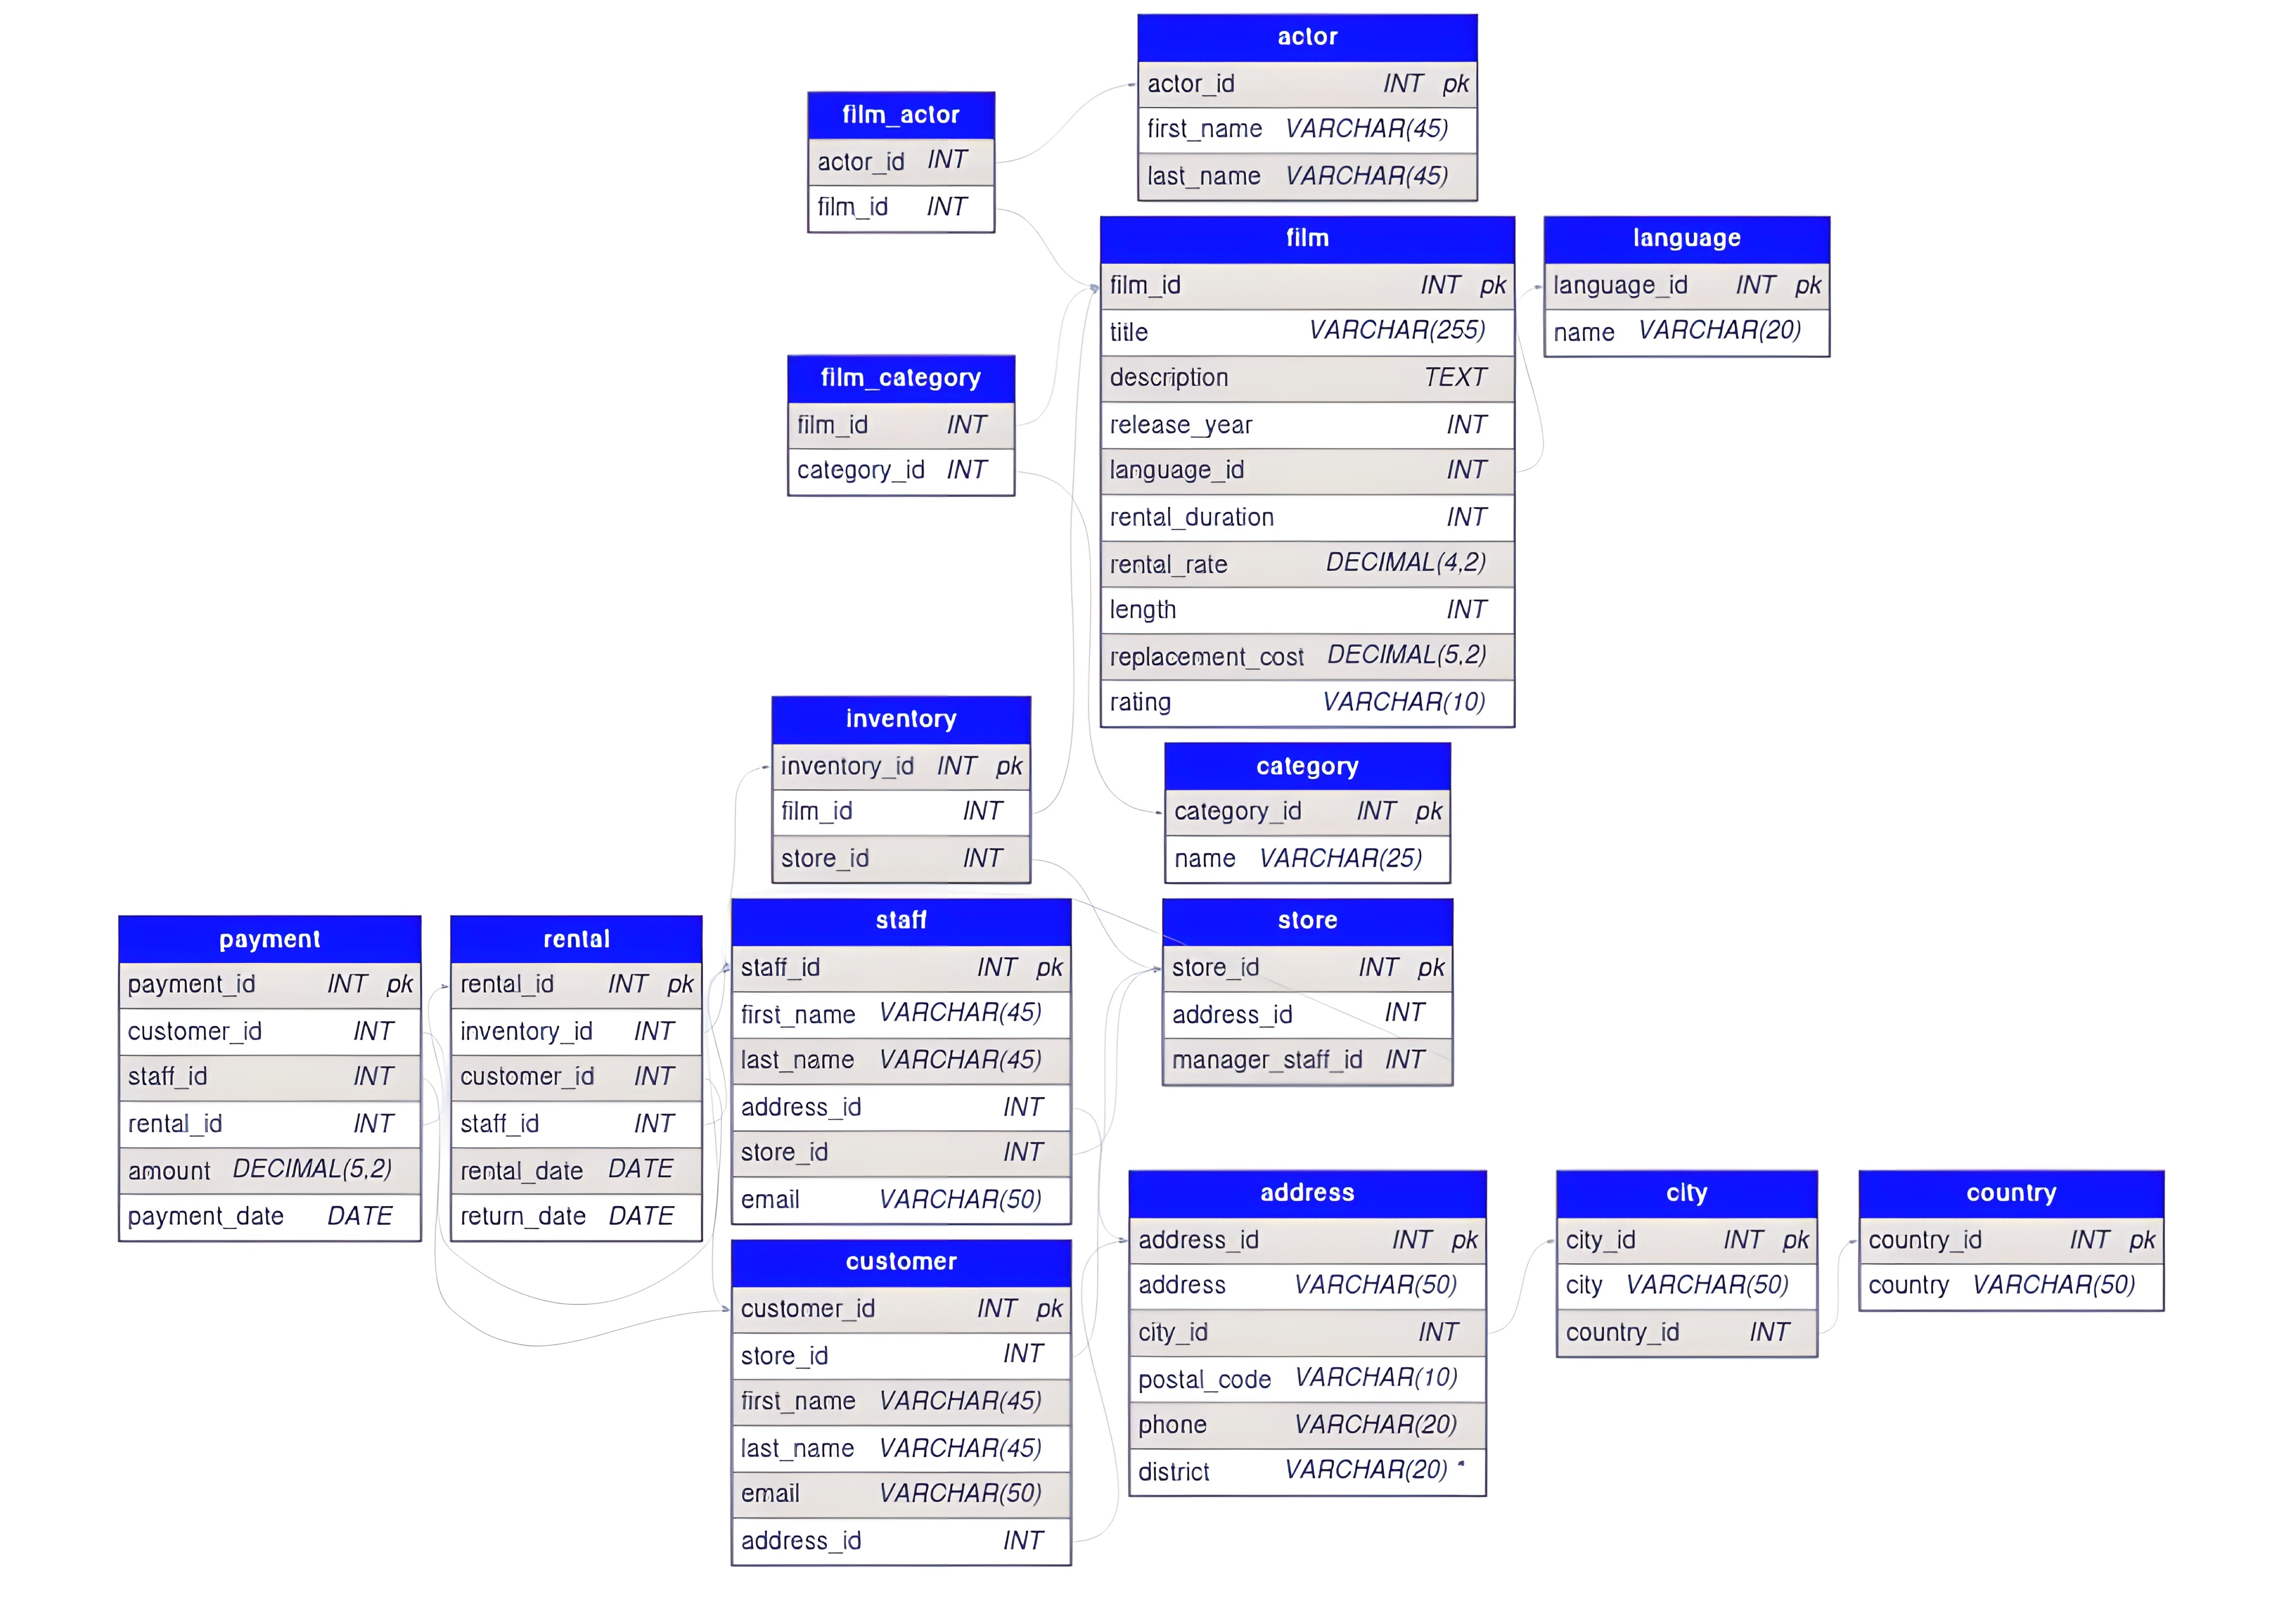
\includegraphics[width=\linewidth]{lab_08_dvdrental_1.png}
\end{figure}

\begin{enumerate}

\item List all addresses where the postal code is either missing or empty.
\ifshowsolutions
\begin{lstlisting}[language=SQL]
SELECT address_id, address, city_id
FROM address
WHERE postal_code IS NULL OR postal_code = '';
\end{lstlisting}
\fi

\item Show cities where the number of residents exceeds a two-digit threshold.
\ifshowsolutions
\begin{lstlisting}[language=SQL]
SELECT ci.city, COUNT(c.customer_id) AS customer_count
FROM customer c
JOIN address a ON c.address_id = a.address_id
JOIN city ci ON a.city_id = ci.city_id
GROUP BY ci.city
HAVING COUNT(c.customer_id) > 99;
\end{lstlisting}
\fi

\item List the titles of films that have never been rented by any customer.
\ifshowsolutions
\begin{lstlisting}[language=SQL]
SELECT f.title
FROM film f
WHERE f.film_id NOT IN (
    SELECT DISTINCT i.film_id
    FROM inventory i
    JOIN rental r ON i.inventory_id = r.inventory_id
);
\end{lstlisting}
\fi

\item Find customers who currently have at least one active rental (i.e., return\_date is NULL).
\ifshowsolutions
\begin{lstlisting}[language=SQL]
SELECT DISTINCT c.first_name, c.last_name
FROM customer c
JOIN rental r ON c.customer_id = r.customer_id
WHERE r.return_date IS NULL;
\end{lstlisting}
\fi

\item List addresses that are not associated with any customer.
\ifshowsolutions
\begin{lstlisting}[language=SQL]
SELECT a.address_id, a.address
FROM address a
LEFT JOIN customer c ON a.address_id = c.address_id
WHERE c.customer_id IS NULL;
\end{lstlisting}
\fi

\item Show the first and last names of customers who live in the city \texttt{London}.
\ifshowsolutions
\begin{lstlisting}[language=SQL]
SELECT c.first_name, c.last_name
FROM customer c
JOIN address a ON c.address_id = a.address_id
JOIN city ci ON a.city_id = ci.city_id
WHERE ci.city = 'London';
\end{lstlisting}
\fi

\item Display rental IDs and rental dates for rentals made after 1 January 2006.
\ifshowsolutions
\begin{lstlisting}[language=SQL]
SELECT rental_id, rental_date
FROM rental
WHERE rental_date > '2006-01-01';
\end{lstlisting}
\fi

\item Find the rental(s) that had the maximum rental duration (return date minus rental date) in days.
\ifshowsolutions
\begin{lstlisting}[language=SQL]
SELECT rental_id, return_date - rental_date AS duration_days
FROM rental
WHERE return_date IS NOT NULL AND return_date - rental_date = (
    SELECT MAX(return_date - rental_date)
    FROM rental
    WHERE return_date IS NOT NULL
);
\end{lstlisting}
\fi

\item List film categories whose total number of rentals exceeds the average rentals per category.
\ifshowsolutions
\begin{lstlisting}[language=SQL]
SELECT c.name, COUNT(*) AS total_rentals
FROM category c
JOIN film_category fc ON c.category_id = fc.category_id
JOIN inventory i ON fc.film_id = i.film_id
JOIN rental r ON i.inventory_id = r.inventory_id
GROUP BY c.name
HAVING COUNT(*) > (
    SELECT AVG(rental_count)
    FROM (
        SELECT COUNT(*) AS rental_count
        FROM film_category fc2
        JOIN inventory i2 ON fc2.film_id = i2.film_id
        JOIN rental r2 ON i2.inventory_id = r2.inventory_id
        GROUP BY fc2.category_id
    ) t
);
\end{lstlisting}
\fi

\item For each film category, display the film that has been rented the most times. 
    
\ifshowsolutions
\begin{lstlisting}[language=SQL]
SELECT c.name AS category, f.title, COUNT(*) AS rental_count
FROM category c
JOIN film_category fc ON c.category_id = fc.category_id
JOIN film f ON fc.film_id = f.film_id
JOIN inventory i ON f.film_id = i.film_id
JOIN rental r ON i.inventory_id = r.inventory_id
GROUP BY c.category_id, c.name, f.film_id, f.title
HAVING COUNT(*) >= ALL (
    SELECT COUNT(*)
    FROM film_category fc2
    JOIN inventory i2 ON fc2.film_id = i2.film_id
    JOIN rental r2 ON i2.inventory_id = r2.inventory_id
    WHERE fc2.category_id = c.category_id
    GROUP BY fc2.film_id
);
\end{lstlisting}
\fi

\end{enumerate}

\end{document}
